% !Mode:: "TeX:UTF-8"


\chapter{绪论}
\label{ch:intro}

本章首先从社会关系的相关概念出发,引出视觉关系的检测问题,以及本文提出的社会关系图谱。本章分析对比了场景图谱与社会关系图谱的不同点,并且简要介绍了当前社会关系检测的工作的研究现状以及它们的特点。最后说明本文的研究动机以及对社会关系理解问题所提出的解决方案以及实验结果。
\section{研究背景和意义}

每个人的社会关系构成了我们日常生活中社会结构的基础。自然的,我们可以利用一个人所在场景的社会关系来理解和解释当前的场景。社会学研究表明,这种对人的社会理解助于对其特征和可能的行为进行推断。当前,我们的社交生活很大部分是在社交媒体上,例如Facebook、Twitter、微信和微博等包含多模态信息的应用,人们会通过文字、视频和音频等媒介含蓄的留下一些与他人关联的痕迹,但是我们能明确的通过分析这些多模态的信息来捕捉他们的社会关系。随着科技的快速发展,智能和潜在的自主系统会成为我们的帮手和同事,我们希望它们不仅可以熟练的完成任务,还希望他们能够融入和在我们人类生活的不同情况下采取适当的行动。此外,通过更好地了解这些隐藏信息,我们希望告知用户潜在的隐私风险。理解社会关系也有助于避免潜在的隐私风险,通过自动分析可能在文本等许多媒体中揭示社会关系的信息并告知用户这一点。在这个模式中,任务要求社会关系的概念和模式需要在生活和的所有方面共同努力,以便从一种感觉到具体的输入输出。虽然已经开始努力解决这一具有挑战性的问题,但社会生活的巨大多样性和复杂性阻碍了进展。最常见的,识别社会关系的计算模型仅仅限定于少数特定的类别。

在图像理解任务上,视觉概念识别获得了越来越多的研究者的关注,包括视觉属性和视觉关系\cite{lu2016visual}。
视觉关系和视觉属性检测的主要目的是生成场景图谱,场景图谱(scene graph)\cite{johnson2015image}是对图片进行描述的一种半结构化的形式,场景图谱是由视觉三元组构成,并且包括关系三元组和属性三元组。场景图谱已经成为计算机视觉和人工智能领域的重要基础资源,因此如何自动的生成场景图谱成为了重要关注点,以利用自然语言信息的\cite{lu2016visual}为代表的工作,代表场景图谱自动生成领域取得了极大的进展。因此,社会属性和社会关系\cite{wang2010seeing} 对于场景理解同样重要。并且本文主要聚焦在解决社会关系检测问题上,并且可以从场景图谱的生成借鉴有用的思想。
给定一张图片,社会关系理解的目的是推断在当前图片这个场景下人之间的社会关系是社会关系检测的准确描述。除了前面提的用处,理解图像场景中这样的关系能帮助现有的算法产生更好的场景描述。例如在图\ref{fig:intro-example}中的第一个样例,用正常的文字来描述的话,`` 一个妇人和女孩正在吃饭''。但是对于社会关系的这个问题下,可以认为是``一个母亲和女儿正在吃饭''。
\begin{figure}[htpb]
	\centering
	%	\includegraphics[width=0.48 \textwidth, trim=10 10 10 80,clip]{./pic/example_new.pdf}
	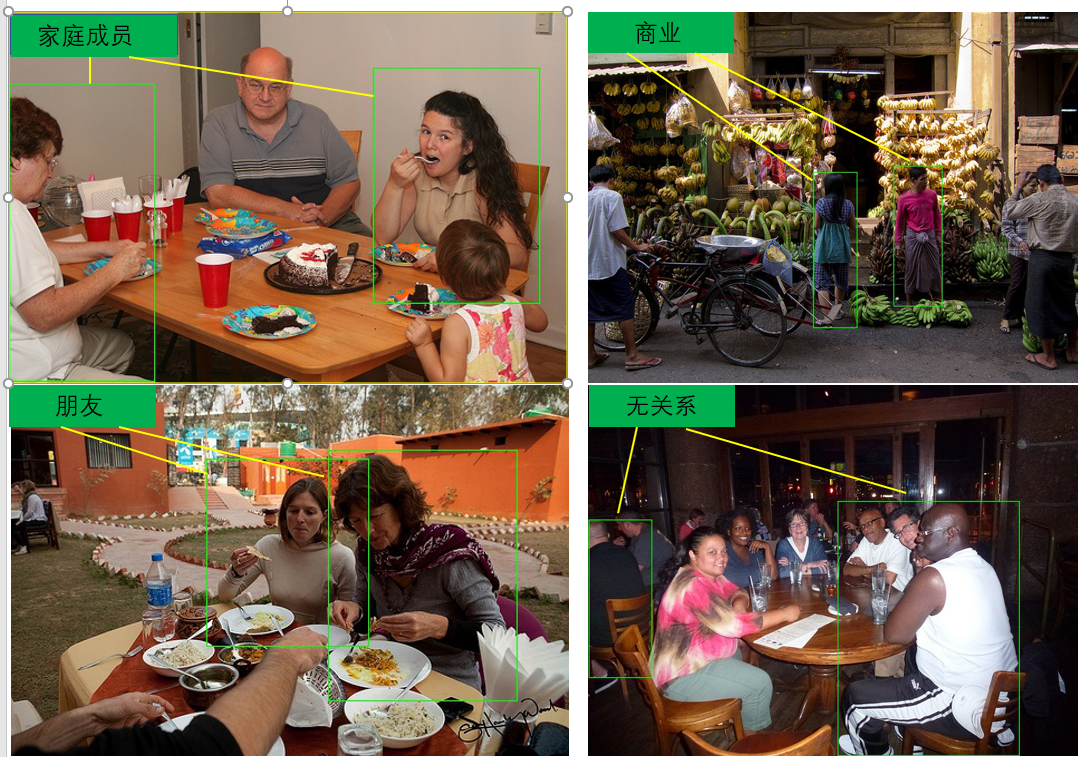
\includegraphics[width=0.95 \textwidth,clip]{example-1.png}
	%\hspace{0.02\textwidth}
	%\vspace*{-0.08cm}
    \caption{PISC数据集中的一些图片例子}
	\vspace*{-3.5mm}
	\label{fig:intro-example}
\end{figure}
\looseness=-1

如何准确的理解社会关系成为研究者需要攻克的课题。一方面,一张图片的社会关系可以通过众包的方式,人工标注得到,比如现有的数据集PISC\cite{li2017dual-glance}和PISC-relation\cite{sun2017a}。当然,自动端到端的方法包括基于人脸特征、年龄、人的头部特征等特征信息的\cite{sun2017a,zhang2015learning}。还有利用周边环境的信息的模型\cite{li2017dual-glance,wang2018deep},这些模型通常需要一个物体检测器或者检测器中RPN(region proposal network),这都是需要引入额外的标注框或者预训练模型。也有通过对周边物体和社会关系共现的统计,例如{\it computer} 和{\it professional}共同出现的概率较大,如果识别出存在{\it computer},那么当前的关系很大概率是{\it professional},通过神经网络引入这些先验知识来提升预测的准确率。这些自动识别社会关系的模型虽然不断在进步,但是从实验结果来看,他们与人工标注的准确率还是存在很大鸿沟,离实际的应用还存在很大的距离。

此外,现有的学习模型大都倾向于挖掘内部的信息或引入外部的知识来辅助理解图片的社会关系场景,但是得到这些外部知识需要额外的人工干预,这是一件耗时耗力的工作,或者一些统计得到的先验知识同样包含一些噪音,这也直接引出了到底是否应该引入这些信息的问题。例如是否利用周边物体的信息,以及如何在缺乏这些信息的情况下取得好的实验效果。受到场景图谱生成的启发,场景图谱的概念最初是在2015年由Johnson 等人\cite{johnson2015image}提出的,是用于描述图片的一种新的半结构化的方式,基本组成单位是视觉三元组,形式为(头实体,关系,尾实体)。受到该领域下Xu(2017)\cite{xu2017scene}的工作首先将整张图片输入,考虑到图片中不同视觉三元组之间的相互影响。例如,当知道`` 马在草地上''倾向于提高检测到`` 人骑着马''这条视觉三元组。对于社会关系检测的场景,如果图片中包含三个人对,其中两个人对的社会关系是``朋友'',那么第三条关系的的社会关系会倾向也是``朋友''或者其他的亲密关系,而不是`` 无关系''。直观上来说,这个是成立的,因此我们可以利用这当前场景下的其他的关系的来推理出当前的关系。

本论文主要研究如何将前文提到的关系场景的上下文信息引入社会关系理解的框架中。本文的出发点完全区别于Li(2017)\cite{li2017dual-glance}、
Wang(2018)\cite{wang2018deep}、以及Zhang等人(2019)\cite{zhang2019multi}。
,对于关系特征的提取方法采用和Li\cite{li2017dual-glance}相同的策略。论文的切入点如图例\ref{fig:intro-example-2},图上六个人对的关系有五对是``朋友''关系,其中只有一对``奶奶-孙女''的关系,因此当前的图片应该是一个朋友聚会的场景拍下的。如果我们想推理出其中一个人对的关系并且已经知道其他部分人对的关系,那么直观的,我们会通过对已经知道的关系进行一个场景的判断,从而推理当前人对的关系到底是什么。在当前例子中,如果已经知道了2对或者3对都是``朋友''关系,那么当前的人对大概率也是``朋友''关系。因此,类似于前文提到的场景图谱的生成,以及现有的社会关系理解的研究现状,将本文工作定义为社会关系图谱生成(social relationship graph generation),一个新的视觉社会关系场景的结构化表示。
\begin{figure}[htpb]
	\centering
	%	\includegraphics[width=0.48 \textwidth, trim=10 10 10 80,clip]{./pic/example_new.pdf}
	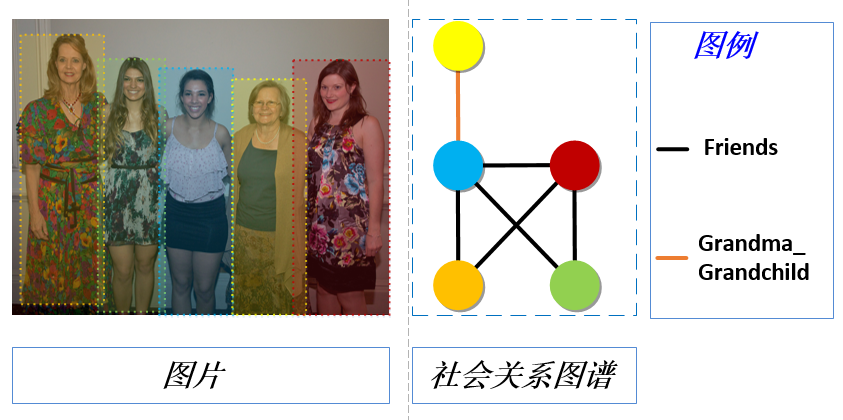
\includegraphics[width=0.95 \textwidth,clip]{example.png}
	%\hspace{0.02\textwidth}
	%\vspace*{-0.08cm}
    \caption{本论文动机的示例图,该图片来自PIPA-relation数据集,其中图片中对应阴影颜色的人对应社会关系图的部分,图上节点间的边表示他们之间的社会关系}
	\vspace*{-3.5mm}
	\label{fig:intro-example-2}
\end{figure}
\looseness=-1

在上述的介绍中,我们分别提到了两方面的相关内容,一方面社会关系理解的意义和作用,另外提到了与社会关系同属视觉理解领域的场景图谱的生成,收到这些工作的影响,可以列出他们的共性和特性如下:
\begin{enumerate}
    \item 场景图谱的基本组成是视觉三元组,社会关系图中是人对和人对间的社会关系,但是场景图谱中并没有人的的类别的概念,社会关系图中节点间的社会关系与人的类别无关。
    \item 场景图谱中的关系类别较多,有80-100个类别,但是在社会关系中,现有数据集不同粒度的关系类别分别为3、6、16,数量上远远不一样。并且在场景图谱中,关系的类型主要以空间关系为主,少量含有语义的关系,但是在社会关系图中,除了{\it No Relation}和空间存在较大关联,其他的均为语义的关系。
    \item 与现有研究工作的区别是,之前的方法均将同一张图片上的不同人之间的关系割裂来看,但是他们间的关系互相影响,现有的研究工作忽略了这一点。
\end{enumerate}

要想解决社会关系图谱的生成问题,一种可行的方法是借助场景中除了人以外其他的信息,由于现有的数据集并没有标注其中的物体信息,所以需要借助额外的检测模型,但是由于模型的准确率的原因,会引入相当一部分的噪音,我们不能简单的加入这些信息,或者说我们是否需要加入这部分信息。其次是借助场景图谱生成的思想,认为一张图片中所有人对的社会关系不是割裂开的,是一同生成的,并且它们之间是相互影响的,但是由于场景图谱和社会关系图谱的区别,我们需要设计一个在社会关系图谱生成任务下人对关系之间的交互机制。

\section{研究现状}

\subsection{视觉关系理解}
在计算机视觉领域,据目前的调研,视觉关系理解领域主要包括两类任务,分别是社会关系理解和场景图谱的生成。社会关系信息被探索来提升几个常见的任务,例如人的轨迹预测、多目标追踪
\cite{chen2012discovering,qin2012improving}和群体活动识别
\cite{direkoglu2012team,lan2012social,lan2012discriminative}。例如,在Deng等人(2016)\cite{deng2016structure}群体活动识别的任务中,群体活动识别需要推理出图上人之间的结构信息,当前的方法是判断每个个体的动作,并且判断图上人之间的关系。但是由于图片特征的复杂和不确定性,这两个任务都是很有挑战的,推断出图上的结构信息能帮助排除一些未参与群体活动的人,得到更好的预测结果。因此预测这些人之间的社会关系能有助于群体活动识别。如图例\ref{fig:deng-example}所示,利用深度学习模型得到的人的表征和场景的表征后,如果知道了图例中第三个人和另外两个人之间不存在关系的情况下,排除第三个人对任务判断的影响。能更为容易的得出当前的群体活动场景是``waiting''。如Alahi(2016)\cite{alahi2016social}、Robicquet等人(2016)\cite{robicquet2016learning}隐含的引入了社会性的约束来预测符合社会常识规则的人类运动轨迹,利用LSTM网络在序列任务的优越性,同时设计了特殊的池化模块来考虑邻居的运动走向。但是可以通过加入已经识别好的社会关系,即人与人之间的相互作用,当作常识规则来增强对运动轨迹预测鲁棒性和准确率。
\begin{figure}[htpb]
	\centering
	%	\includegraphics[width=0.48 \textwidth, trim=10 10 10 80,clip]{./pic/example_new.pdf}
	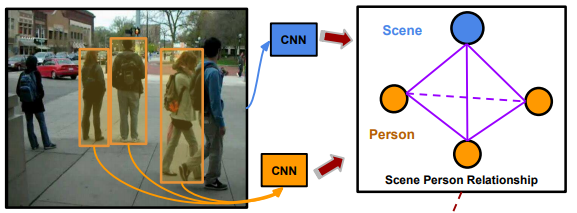
\includegraphics[width=0.95 \textwidth,clip]{deng-example.png}
	%\hspace{0.02\textwidth}
	%\vspace*{-0.08cm}
    \caption{来自Deng等人\cite{deng2016structure}群体活动识别的示例图}
	\vspace*{-3.5mm}
	\label{fig:deng-example}
\end{figure}
\looseness=-1

在社会关系理解之外,也有很多的工作明确的关注社会属性和社会结构的识别Wang等人(2010)\cite{wang2010seeing}通过分析个人的相册集来实现个人的家庭社会关系识别,
亲属关系验证\cite{dibeklioglu2013like,fang2010towards,xia2012understanding}和亲属识别\cite{chen2012discovering,guo2014graph}等任务也被广泛的探索和研究。Zhang等人(2015)\cite{zhang2015learning}研究人的面部表情,例如友好的、统治的,这些信息有助于推断社会关系。而在基于视频分析的领域中,Ding等人\cite{ding2014learning}从电影中挖掘演员的关系。社会关系理解在某个方面和社会信号处理\cite{vinciarelli2009social},社会信号处理的目标是利用多个传感器理解社会信号和社会行为,例如角色识别、影响力排名和统治力检测等\cite{hung2007using,salamin2009automatic}。但是本文关注的社会关系理解本质上不同于前面提到的这些工作,和基于面部表情的社会关系检测不同的是,本文的研究图片中的个体往往是姿态和朝向都不确定的。此外,本文着重的社会关系是更普遍的社会关系,而不是家庭相册中的亲属关系。与视频任务不同的是,本文关注的一张图片中的视觉信息。

前面的社会关系理解的工作大多数都是利用向量化的社会关系来帮助推理,与社会关系理解同属同一个视觉关系理解任务类别,即场景图谱的生成,又或者称为视觉关系检测。该任务的最早是Johnson等人于2015年提出的
\cite{johnson2015image},是一种用于描述图片场景的新的方式,与本文工作不同的是,场景图谱中的主要组成部分不仅包括人,还包括很多日常物体,如图\ref{fig:sg-example}所示。两个工作最核心的挑战在于识别出物体之间的关系。根据图片生成的场景图谱是很多计算机视觉任务的重要输入,Johnson等人(2015)\cite{johnson2015image}提出利用场景图谱来进行图片检索任务,提高了图片检索任务的效果。Zhu等人(2017)\cite{zhu2017knowledge}在视觉问答领域引入场景图谱中的信息,通过在训练过程中引入外部的知识帮助提升问答的效果。Marino(2017)\cite{marino2017the}利用得到场景图谱结合图神经网络提高图片的分类效果。同样是Johnson等人(2018)\cite{johnson2018image}将场景图谱当作输入,利用图卷积神经网络来对场景图片向量化获得物体的结构编码向量,当作特征来预测物体在图片中的包围盒位置和分割掩膜,结合生成对抗网络生成符合场景图谱描述的图片。在以上的工作中,均是利用已生成好的场景图谱当作输入来辅助其它的任务,因此一个完整度更高、越正确的场景图谱自然而然对于提升这些任务的帮助更大。
\begin{figure}[htpb]
	\centering
	%	\includegraphics[width=0.48 \textwidth, trim=10 10 10 80,clip]{./pic/example_new.pdf}
	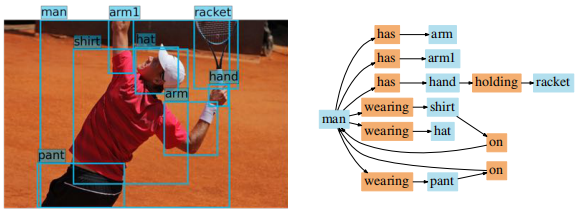
\includegraphics[width=0.95 \textwidth,clip]{sg.png}
	%\hspace{0.02\textwidth}
	%\vspace*{-0.08cm}
    \caption{场景图谱\cite{xu2017scene}的示例图}
	\vspace*{-3.5mm}
	\label{fig:sg-example}
\end{figure}
\looseness=-1

\subsection{关系理解的方法}
在以上关于视觉信息理解的两个方向上,都有大量的工作提出,分别用于解决不同场景的问题。而对于社会关系理解,作为最早的工作,Wang等人(2010)\cite{wang2010seeing}开始引入家庭关系当前背景来识别人之间亲属关系。在后来的工作中
\cite{dibeklioglu2013like,xia2012understanding,chen2012discovering},为了捕获这些社会关系展现出来的一些规律,探索了面部表情和属性等用于亲属关系识别和验证。并且为了促进社会关系理解领域的研究和发展,Li\cite{li2017dual-glance} 和Sun\cite{sun2017a}构建了大规模的数据集,并且利用深度学习的模型直接从图片中学习来识别关系。对于Sun构建的数据集PIPA-Relation,该数据集的关系包括5个关系域,然后基于这5个关系域又划分为16条关系。同样,Li基于关系模型理论,定义了一系列的关系列别,包含两个不同层次关系的划分,粗粒度的3类关系和细粒度的6类关系。在Sun(2017)等人的工作中,不仅提出了两个关系粒度的数据集,而且提出了Dual-glance模型。该模型是一个流水线的模型,并且包括两个模块,主要的的创新点在于利用人对周边的物体信息来提升关系检测的效果。Wang(2018)等人提出了基于知识图谱的深度推理模型,通过图门控神经网络引入物体的社会关系的共现的常识知识来实现物体和关系之间的推理,本质上还是利用周边的物体信息,但是在Dual-glance 中,用到只是周边的物体区域,并不需要准确的识别出物体区域的物体类别。Zhang等人(2019)提出一个多粒度推理框架来实现社会关系检测,作者主要是设计了多个粒度的得分,包括全局得分、人和周边物体的交互图的得分、以及人的姿态图的得分。Zhang等人的模型主要创新点在于引入人的姿态这一特征,并且指出只有从多个粒度的信息层面融合起来才能消除低层次特征到高层次的社会关系理解任务

在关系理解领域,除了社会关系理解,还有视觉关系检测任务。由于场景图谱常用于图片检索\cite{johnson2015image}等任务,因此如何更好的实现视觉理解这个难题自然而然的成为许多研究者想要攻克的难题。与社会关系检测不同,视觉关系检测首先依赖于一个物体检测器识别出所有的物体,然后依次两两识别两个物体存在的关系。在社会关系检测中,物体的类别只有人,并且一张图片中的人往往不会太多。Lu等人\cite{lu2016visual} 提出首先提出VR-P模型,利用自然语言得到的词向量作为先验知识来帮助单条三元组的检测。后来,Zhang 等人\cite{zhang2017visual} 提出VTranE 模型,模拟知识图谱中关系平移性质,本质上还是一个关系的分类器。但是并没有考虑到视觉关系的复杂度,并且不同于自然语言的状态翻译。Li (2017)等人\cite{li2017scene}进一步提出了多任务混合模型,任务包括场景图谱、区域描述生成、物体识别。和VRD类似,通过多种任务联合训练,引入额外的信息。
Zellers 等人(2018)\cite{zellers2018neural}提出motif-net,通过分析数据集得出关视觉关系严重依赖头尾实体的类别,利用双向循环神经网络对物体类别编码信息进行编码处理,提升了物体识别的准确度,进而提升了任务的效果。Xu等人(2017)对于场景图谱进行建模,分别包含物体节点和关系节点,然后采用Message Passing的方式进行迭代。通过相邻的节点或边对目标节点或边进行约束,从而对这些特征进行微调,达到提升的效果。Yang等人(2018)利用图卷积网络进行不同节点之间的Message passing来达到约束的效果,并且提出了新的评价指标。但是在进行Message passing前,假设识别出有$n$个物体,那么存在$n \times (n-1)$个头尾实体对,但是这里面有相当一部分的实体对是显然不成立的,文章提出了一个RelPN网络来生成代表关系的区域,剔除一些显然不成立的实体对,并且有效的减少了模型的复杂度。融合自然语言知识提出的VRD 模型\cite{liang2018visual},本文初始步骤中的特征提取工作中包含空间信息的提取便收到该工作的启发,此外VRD还提出了一个新的损失函数来处理多对多的情况,该损失函数还引入了先验条件概率。

\subsection{研究现状小结}
对于人的轨迹预测、 多目标追踪 和群体活动识别任务,引入社会关系的信息能有效的提高这些任务的效果。当前社会关系理解的工作主要方式是引入额外的信息,例如引入面部表情和属性、年龄等。以及通过物体检测的方法识别出当前场景中的物体,来优化单纯通过提取人的区域的表征。最新的工作通过尝试引入物体和关系间的常识知识来提高模型的效果。无论是采用额外的物体检测模型还是通过引入常识知识,都是外部信息,不可避免的需要额外的消耗或引入一些噪声。因此,如何利用更少的信息,来提升预测效果是当前的一大挑战。同时以消息传递机制为技术栈的微调机制的方法在场景图谱,在一定程度上解决了场景图谱的生成问题。然而,由于场景图谱和社会关系任务理解两者之间的区别,如何在社会关系理解中引入消息传递机制仍然面临很多的挑战。

\section{本文工作}

本文首先通过介绍现有的社会关系理解最新研究工作,分析它们的模型设计的出发点,模型的结构,分析这些工作的忽略的信息,即没考虑到整张图片不同的人对的关系之间的互相影响。因此,本文提出了一个考虑到同一张图片不同关系之间信息交互的模型:包含人对消息传递机制的模型,人对关系网络(Person-pair Relation Network),简称PPRN,最后把该模型应用到社会关系理解的任务中,并且在两个公开数据集上做了对比实验。
本文提出的PPRN模型包括以下模块:
\begin{enumerate}
    \item 在视觉场景的社会关系理解领域,本文首次定义了一个新的结构化表示,社会关系图谱(Social Relationship Graph),并且由以下几个模块来实现社会关系图谱的生成。
    \item 特征抽取模块,对于特征抽取模块,本文采用两个个ResNet101\cite{he2016deep}表示社会关系的图像基本特征。此外,人对的位置信息也提取入了最后的关系编码向量中。
    \item 消息传递模块,本文首次尝试在社会关系理解任务中引入多个人对之间的关系的想法。对于消息传递模块,利用以GRU单元为组件的RNN来实现消息传递,并且设置多个迭代步,实现消息传递和池化模块的交互。采用RNN 最后隐藏层的输出作为图片中人对的关系表征。消息池化模块,本文设计了一个交互机制来处理人对之前的关系的信息,同时利用注意力机制来提高模型的效果。本文设计了一个多任务的损失函数,包括关系分类损失和关系域分类损失,两个分类任务会相互促进,学习到更合适的关系编码。
    \item 融合周边物体信息模块,与Dual-galnce\cite{li2017dual-glance}类似,本文在经过消息传递、池化两个模块后得到的人对关系编码,利用注意力机制得到周边物体区域特征编码。两部分特征融合后,进行最后的关系分类。
\end{enumerate}

在实验中,本文在两个公开数据集上验证了PPRN模型的有效性,它们分别是PIPA-Relation和PISC,其中PISC包括两个粒度的子数据集PISC-coarse和PISC-fine。与此同时,在加入最后的周边物体信息模块后,模型效果轻微下降。
接着,本文进一步通过案例研究的方法分析了PPRN模型的具体效果。从实验结果可以看出,PPRN模型在与其他基准模型的比较中取得了在两个数据集上取得了最优的结果,说明了引入不同关系之间交互的消息传递机制在社会关系理解为基础场景中的重要性。

\section{论文结构}

全文的组织结构描述如下:

第1章:介绍了社会关系理解的相关背景,点明了当前社会关系理解存在的缺点,由此引入了同属视觉关系理解人物的场景图谱,分析并总结了场景图谱的研究现状,并针对两者的共同点引出社会关系理解的提升方案。

第2章:首先介绍了图像领域的视觉信息抽取的方法,从简单的神经网络、卷积神经网络、以及残差网络等介绍。之后基于前面的神经网络的知识,介绍了现有工作中常用的物体检测与识别的方法,并进行了讨论与对比。然后详细介绍了当前社会关系理解模型的各个部件,最后对本章内容进行了总结。

第3章:针对社会关系理解的特点,提出了基于消息传递机制的社会关系理解方法,设计了图像中不同人对的社会关系交互的PPRN模型,并且具体介绍了模型的细节。同时实现了结合周边物体信息的模块,分析了模型的设计原则和具体细节。

第4章:首先介绍了两个在社会关系理解领域常用的数据集,并对PPRN模型在不同关系粒度的数据集上进行了训练和测试,接着针对实验结果进行了分析。然后还进一步通过案例研究的方式分析了PPRN在社会关系理解的变现。

第5章:总结了本文的研究工作,并且提出了进一步的研究展望。



